\documentclass[a4paper,12pt]{article}

\usepackage[T2A]{fontenc}			
\usepackage[utf8]{inputenc}			
\usepackage[english,russian]{babel}	

\usepackage[
bookmarks=true, colorlinks=true, unicode=true,
urlcolor=black,linkcolor=black, anchorcolor=black,
citecolor=black, menucolor=black, filecolor=black,
]{hyperref}

\usepackage{color}
\usepackage{caption}
\DeclareCaptionFont{white}{\color{black}}
\DeclareCaptionFormat{listing}{\colorbox{white}{\parbox{\textwidth}{#1#2#3}}}
\captionsetup[lstlisting]{format=listing,labelfont=white,textfont=white}

\usepackage{amsmath,amsfonts,amssymb,amsthm,mathtools} 
\usepackage{wasysym}

\usepackage{graphicx}
%\usepackage[cache=false]{minted}
\usepackage{cmap}
\usepackage{indentfirst}

\usepackage{listings} 
\usepackage{fancyvrb}

\usepackage{geometry}
\geometry{left=2cm}
\geometry{right=1.5cm}
\geometry{top=1cm}
\geometry{bottom=2cm}

\setlength{\parindent}{5ex}
\setlength{\parskip}{0.5em}

\usepackage{pgfplots}
\usetikzlibrary{datavisualization}
\usetikzlibrary{datavisualization.formats.functions}

\begin{document}
	\lstset{ %
		language=C,                 % выбор языка для подсветки (здесь это С)
		basicstyle=\small\sffamily, % размер и начертание шрифта для подсветки кода
		numbers=left,               % где поставить нумерацию строк (слева\справа)
		numberstyle=\tiny,           % размер шрифта для номеров строк
		stepnumber=1,                   % размер шага между двумя номерами строк
		numbersep=5pt,                % как далеко отстоят номера строк от подсвечиваемого кода
		backgroundcolor=\color{white}, % цвет фона подсветки - используем \usepackage{color}
		showspaces=false,            % показывать или нет пробелы специальными отступами
		showstringspaces=false,      % показывать или нет пробелы в строках
		showtabs=false,             % показывать или нет табуляцию в строках
		frame=single,              % рисовать рамку вокруг кода
		tabsize=2,                 % размер табуляции по умолчанию равен 2 пробелам
		captionpos=t,              % позиция заголовка вверху [t] или внизу [b] 
		breaklines=true,           % автоматически переносить строки (да\нет)
		breakatwhitespace=false, % переносить строки только если есть пробел
		escapeinside={\%*}{*)}   % если нужно добавить комментарии в коде
	}

\begin{figure}[h!]
	\begin{center}
		{
\includegraphics[width = \textwidth]{titul.jpg}}
	\end{center}
\end{figure}

%\vspace*{10mm}

\huge
\begin{center}
	Лабораторная работа №2
\end{center}

\vspace*{10mm}

\large
\begin{center}
	Тема: <<Задача Коши для системы из двух уравнений ОДУ>>
\end{center}

\vspace*{20mm}

\large
\begin{flushleft}
	Студент: Левушкин И.К. \\
	Группа: ИУ7-62Б \\
	Оценка (баллы): \\
	Преподаватель: Градов В.М.
\end{flushleft}

\vspace*{50mm}

\large
\begin{center}
	Москва, 2020 г.
\end{center}

\thispagestyle{empty}

\newpage

\section{Условие задачи}

Рассмотрим следующую электрическую схему:
\begin{figure}[h!]
	\begin{center}
		{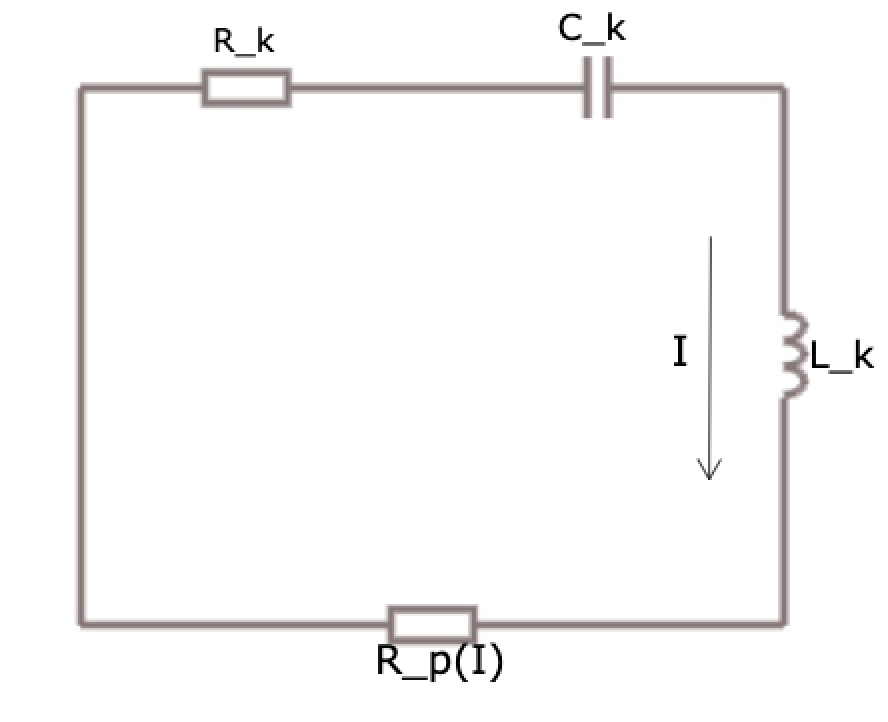
\includegraphics[scale = 0.4]{chain.jpg}}
		\label{chain}
	\end{center}
\end{figure}

Начальные условия:
\begin{itemize}
	\item $t = 0$
	\item $I = I0$
	\item $U_c = U_c0$
\end{itemize}

Обход цепи по второму правилу Кирхгофа:
\[L_k \frac{dI}{dt} + (R_k + R_p(I)) I - U_c = 0\]

Где
\[Где R_p(I) = \frac{L_e}{2\pi R^2 \int_{0}^{1} \sigma(T(z)) zdz}\]



По определению конденсатора:
\[C_k \frac{dU_c}{dt} = -I\]

Итого, имеем систему из двух уравнений ОДУ:
\[
\left\{
\begin{aligned}
U'(t) &= -\frac{I}{C_k} \\
I'(t) &= \frac{U_c - (R_k + R_p(I)) I}{L_k} \\
\end{aligned}
\right.
\]

\section{Метод решения задачи}

В качестве решения будем использовать численный явный метод - Рунге-Кутта, имеющий 4-ый порядок точности.

\subsection{Преимущества схем Рунге-Кутта}
\begin{itemize}
	\item схемы явные
	\item формулы достаточно точные
	\item позволяют вести расчеты с n-ым шагом
\end{itemize}

\subsection{Рунге-Кутт 4-ого порядка точности}

Ниже приведены формулы обобщенной схемы Рунге-Кутта для двух переменных

\[
\left\{
\begin{aligned}
	U'(x) &= f(x, U, V) -> y \\
	V'(x) &= \phi(x, U, V) -> z \\
	V(\eta) &= V_0 \\
	U(\eta) &= U_0 \\
\end{aligned}
\right.
\]

\[y_{n+1} = y_n + \frac{k_1 + 2k_2 + 2k_3 + k_4}{6}\]
\[z_{n+1} = z_n + \frac{q_1 + 2q_2 + 2q_3 + q_4}{6}\]
Где 
\begin{itemize}
	\item $k_1 = h_n f(x_n, y_n, z_n)$, $q_1 = h_n \phi(x_n, y_n, z_n)$
	\item $k_2 = h_n f(x_n + \frac{h_n}{2}, y_n + \frac{k_1}{2}, z_n + \frac{q_1}{2})$, $q_2 = h_n \phi(x_n + \frac{h_n}{2}, y_n + \frac{k_1}{2}, z_n + \frac{q_1}{2})$
	\item $k_3 = h_n f(x_n + \frac{h_n}{2}, y_n + \frac{k_2}{2}, z_n + \frac{q_2}{2})$, $q_3 = h_n \phi(x_n + \frac{h_n}{2}, y_n + \frac{k_2}{2}, z_n + \frac{q_2}{2})$
	\item $k_1 = h_n f(x_n + h_n, y_n + k_3, z_n + q_3)$, $q_1 = h_n \phi(x_n + h_n, y_n + k_3, z_n + q_3)$
\end{itemize}


\newpage
\section{Использованные константы}


\begin{figure}[h!]
	\begin{center}
		{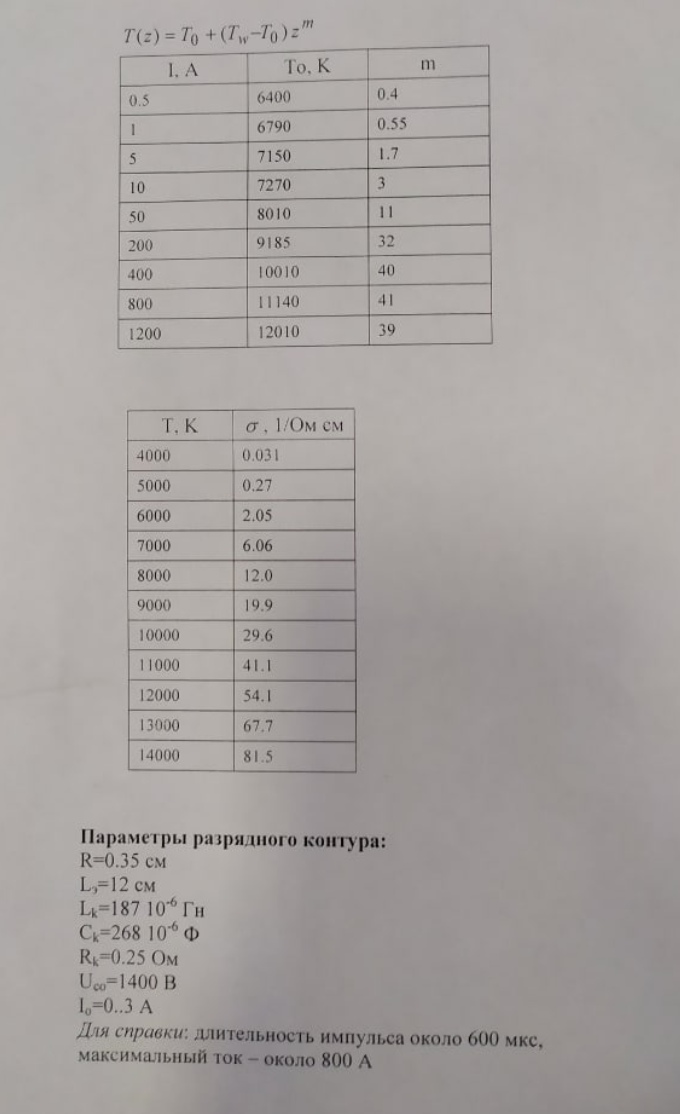
\includegraphics[scale = 0.4]{const.jpg}}
		\label{const}
	\end{center}
\end{figure}

$T_w = 2000$

\newpage
\section{Пример работы программы}

Ниже приведен пример работы программы при $R_k + R_p = 0$ (идеальные условия, без потерь); при шаге $h = 10$ мкс, $t_{max} = 10000$ мкс, $t_{min} = 0$ мкс

\begin{figure}[h!]
	\begin{center}
		{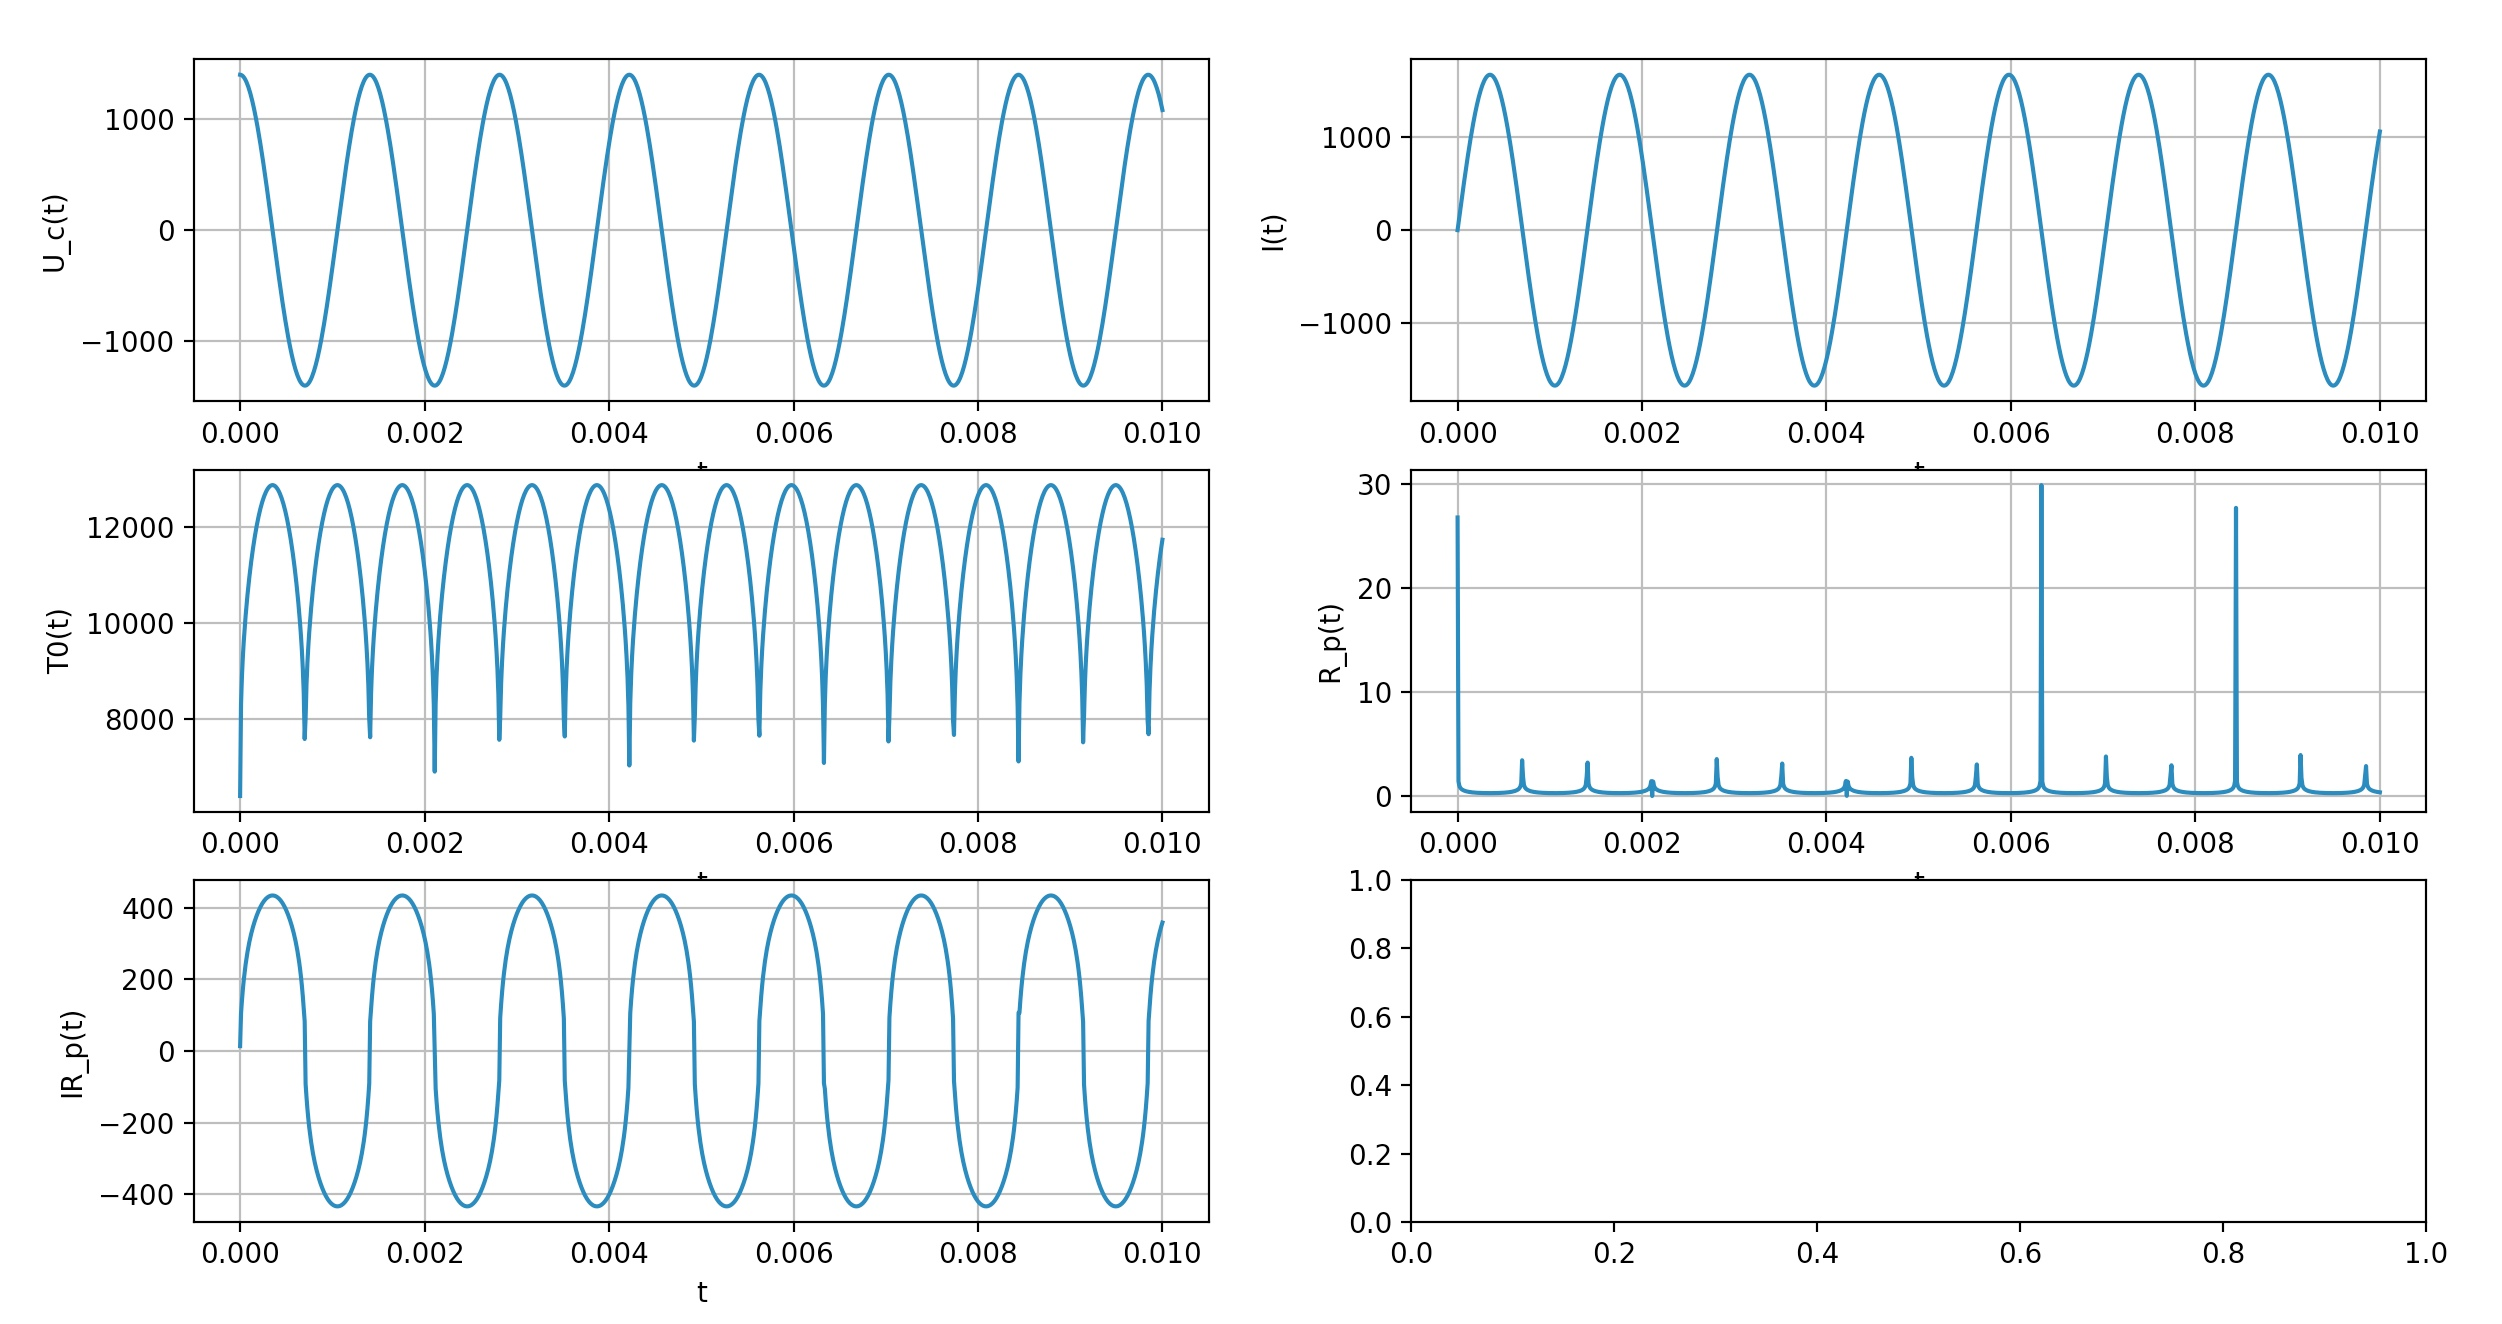
\includegraphics[scale = 0.2]{RkRp.jpg}}
		\label{RkRp}
	\end{center}
\end{figure}


Ниже приведен пример работы программы при шаге $h = 10$ мкс, $t_{max} = 10000$ мкс, $t_{min} = 0$ мкс, $R_k = 0.35 $ Ом.
\begin{figure}[h!]
	\begin{center}
		{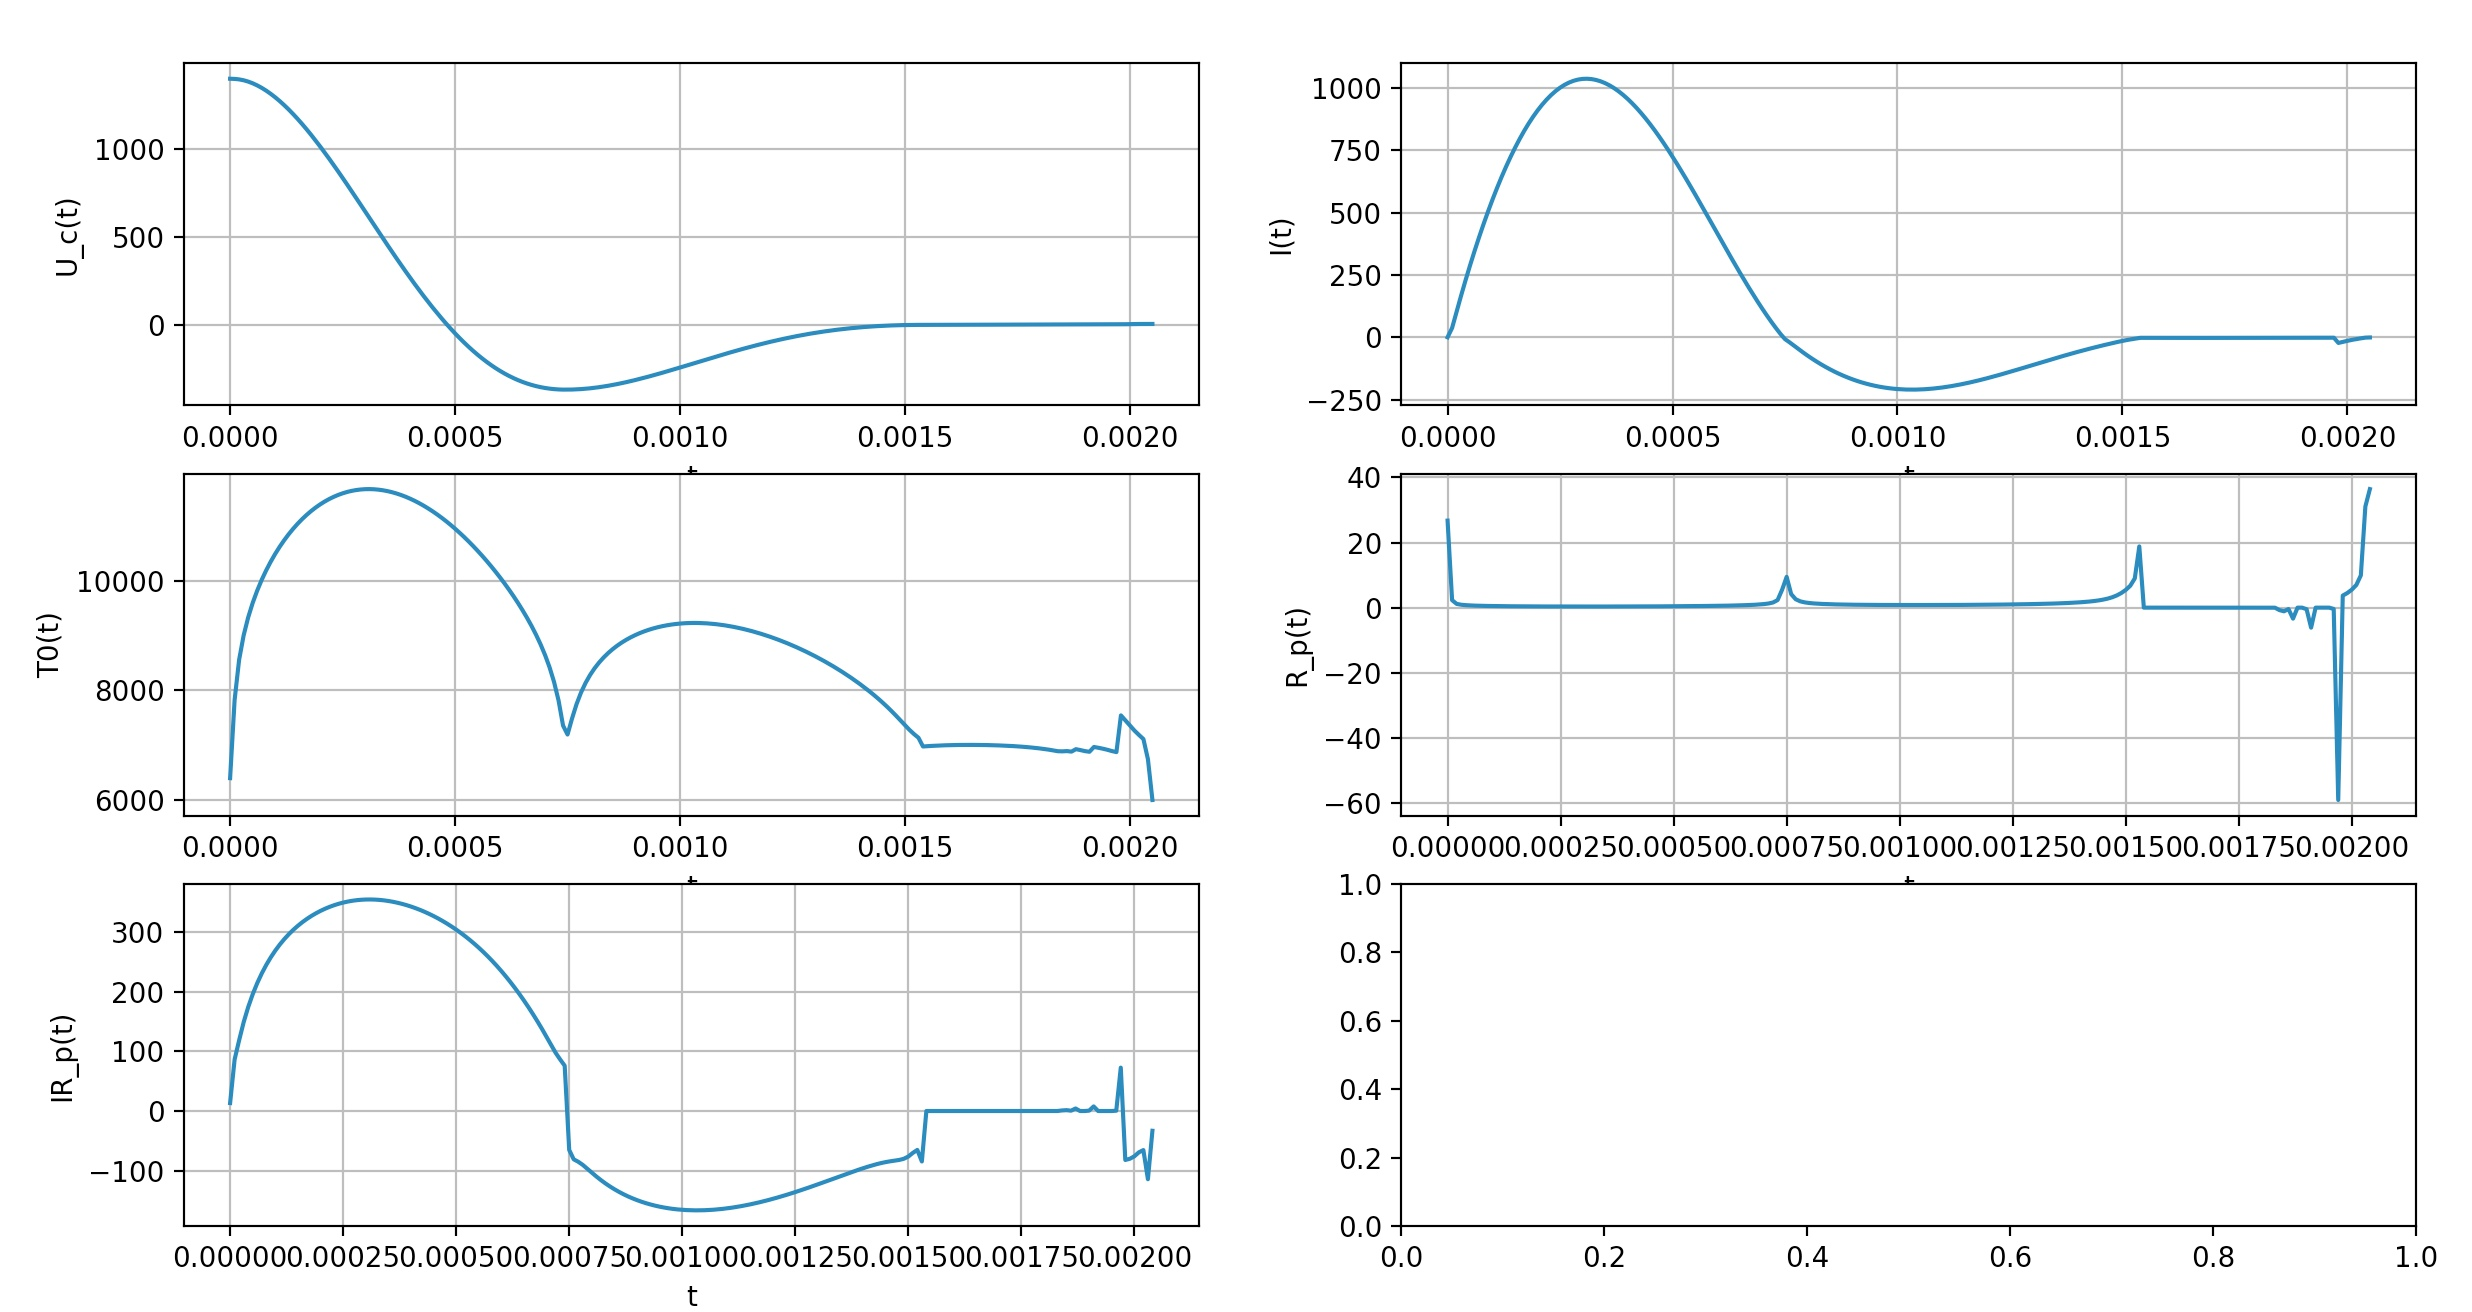
\includegraphics[scale = 0.2]{10000.jpg}}
		\label{10000}
	\end{center}
\end{figure}


\newpage
Ниже приведен пример работы программы при шаге $h = 10$ мкс, $t_{max} = 700$ мкс, $t_{min} = 0$ мкс, $R_k = 0.35 $ Ом.

\begin{figure}[h!]
	\begin{center}
		{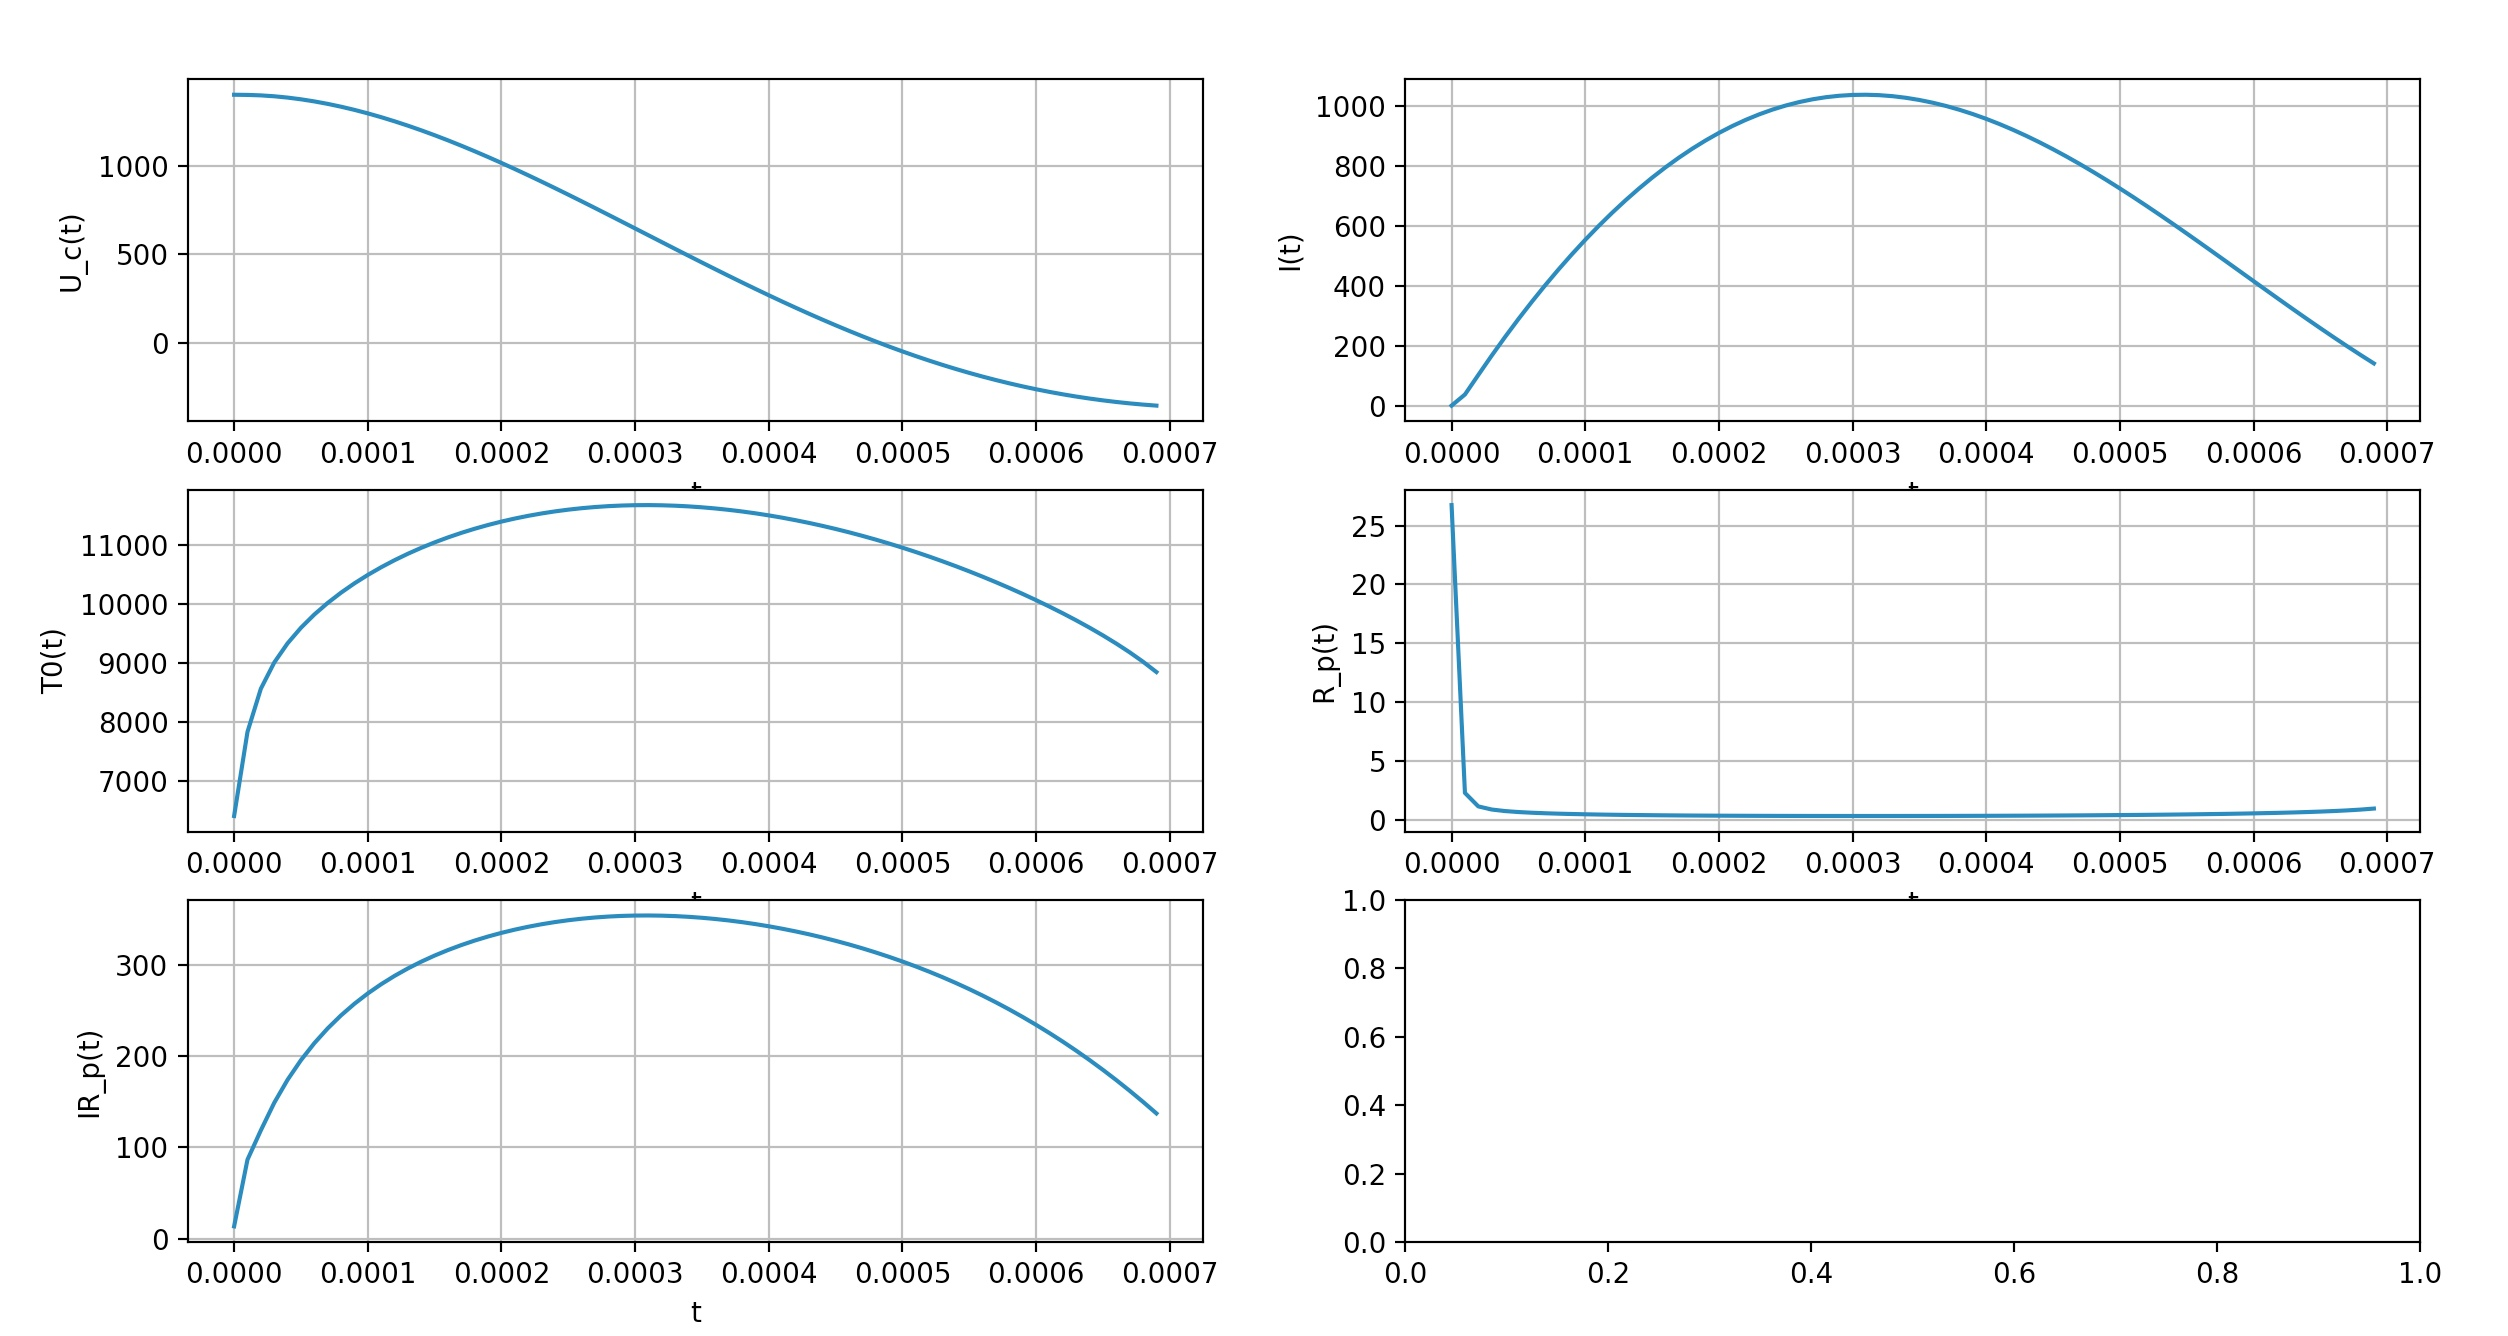
\includegraphics[scale = 0.2]{700.jpg}}
		\label{700}
	\end{center}
\end{figure}

Ниже приведен пример работы программы при шаге $h = 10$ мкс, $t_{max} = 2000$ мкс, $t_{min} = 0$ мкс, $R_k = 3.0 $ Ом.

\begin{figure}[h!]
	\begin{center}
		{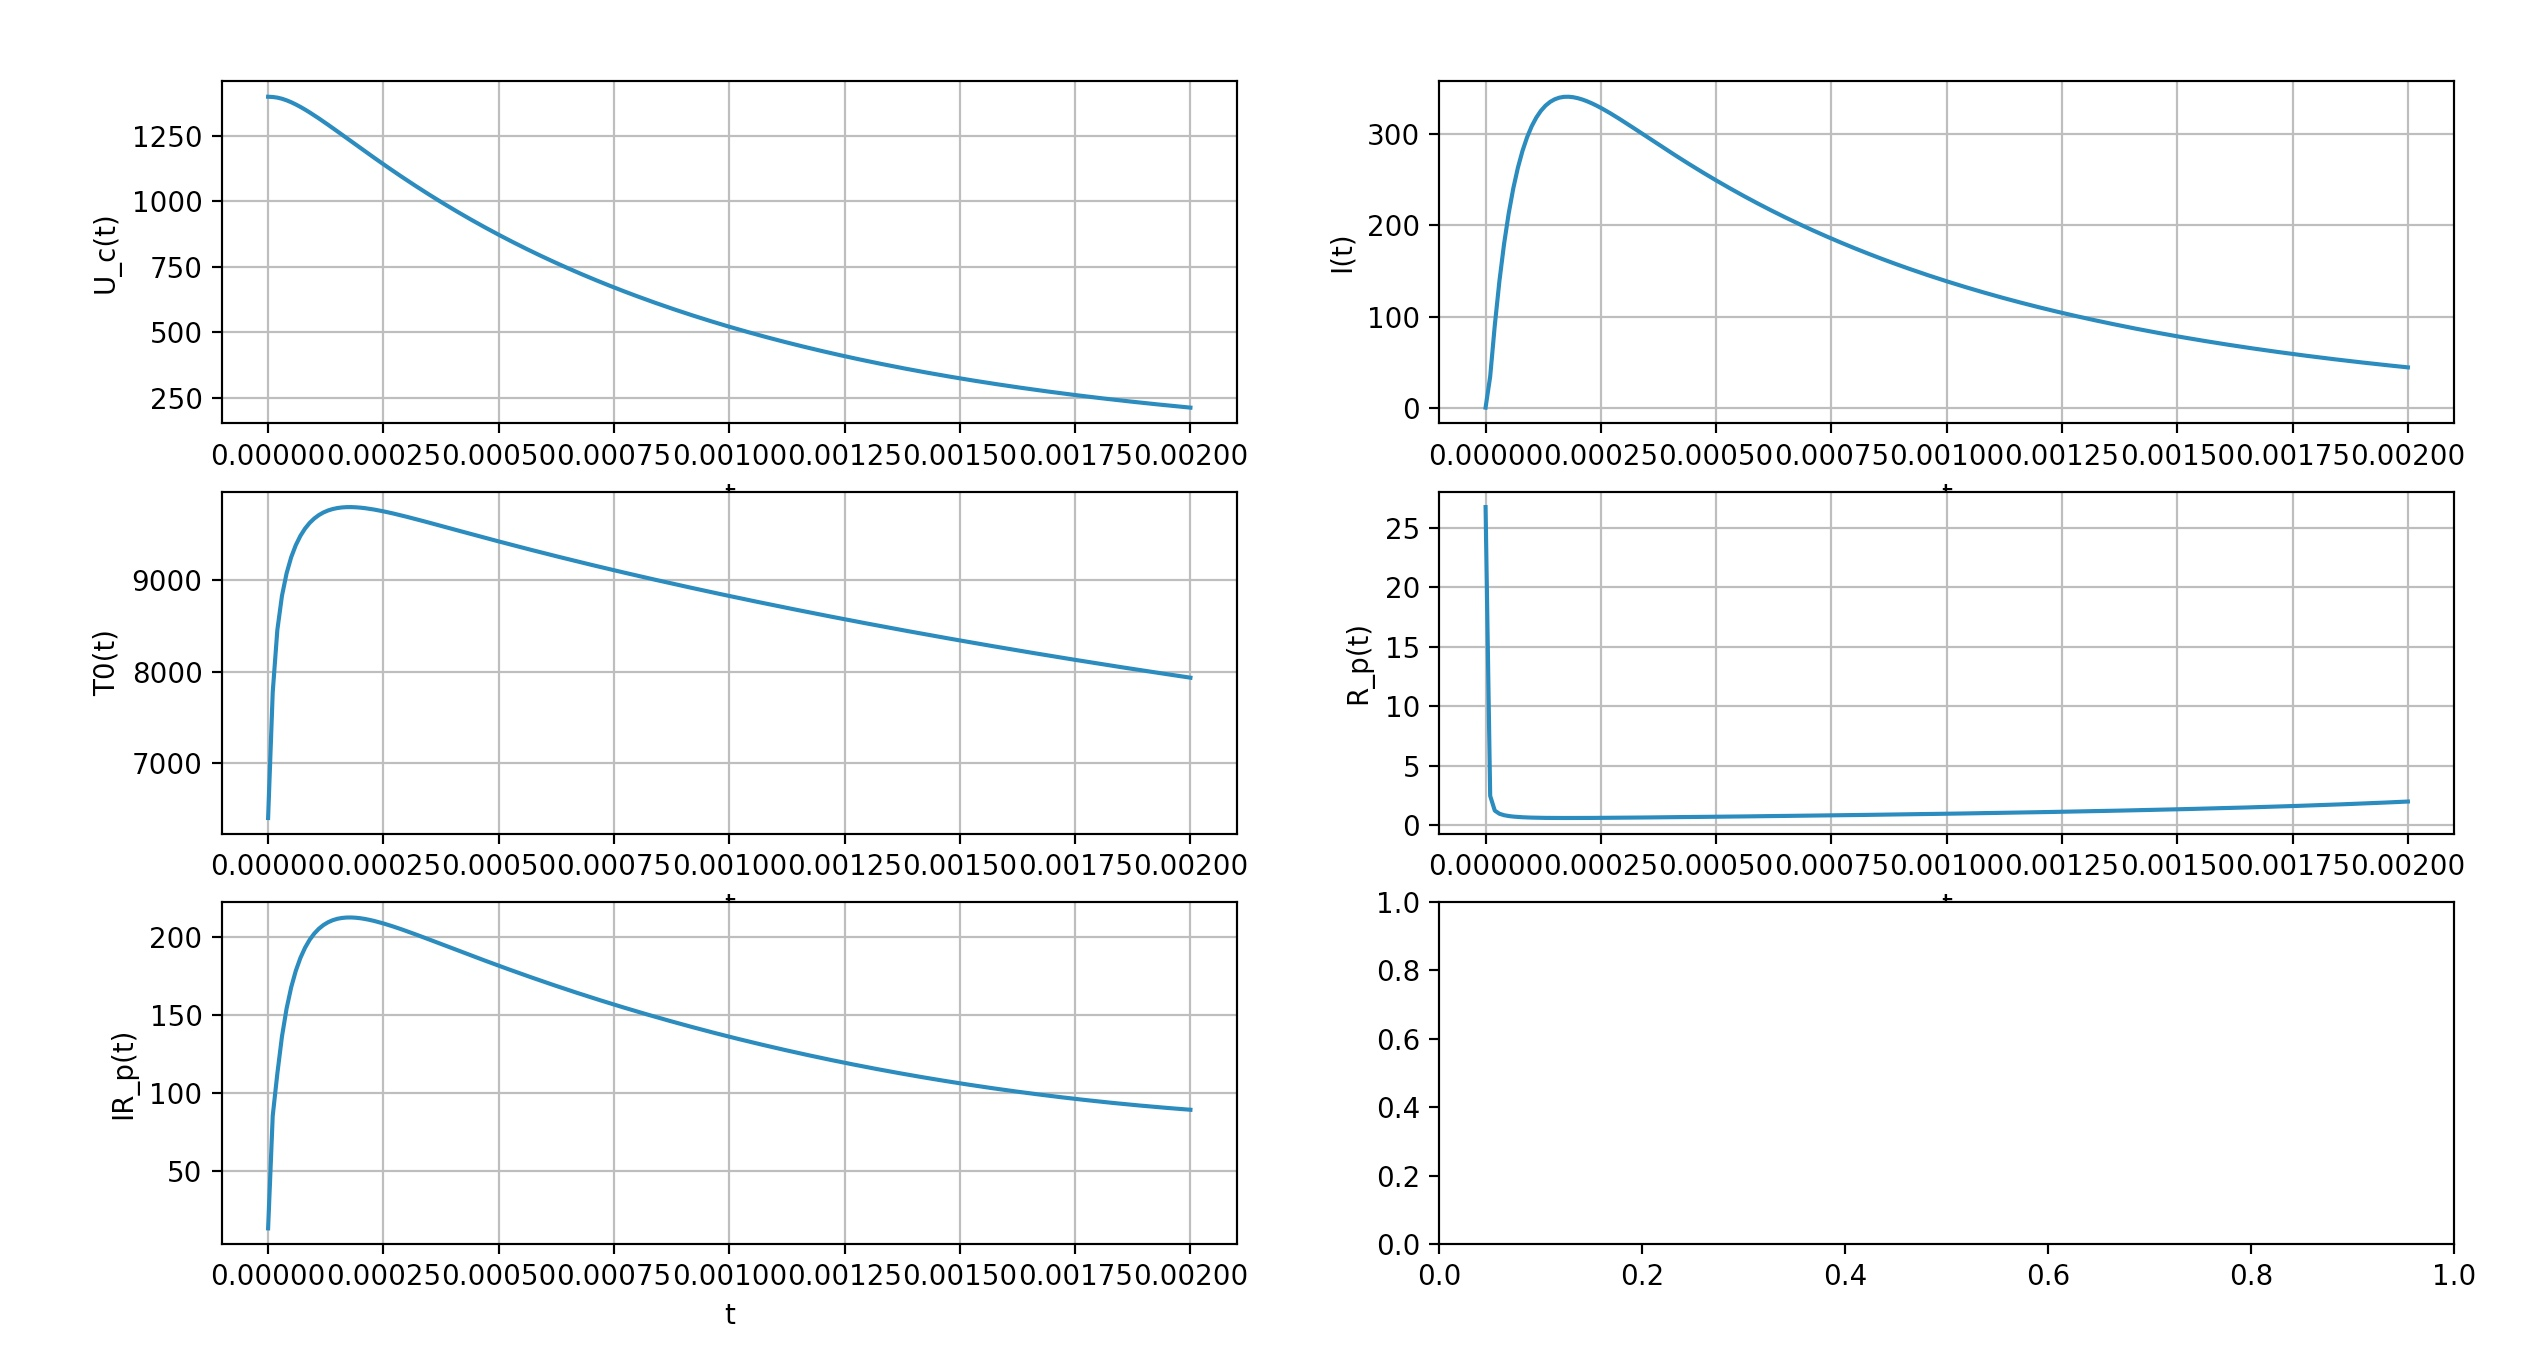
\includegraphics[scale = 0.2]{2000.jpg}}
		\label{700}
	\end{center}
\end{figure}

Ниже приведен пример работы программы при шаге $h = 10$ мкс, $t_{max} = 10000$ мкс, $t_{min} = 0$ мкс, $R_k = 0.0 $ Ом.

\begin{figure}[h!]
	\begin{center}
		{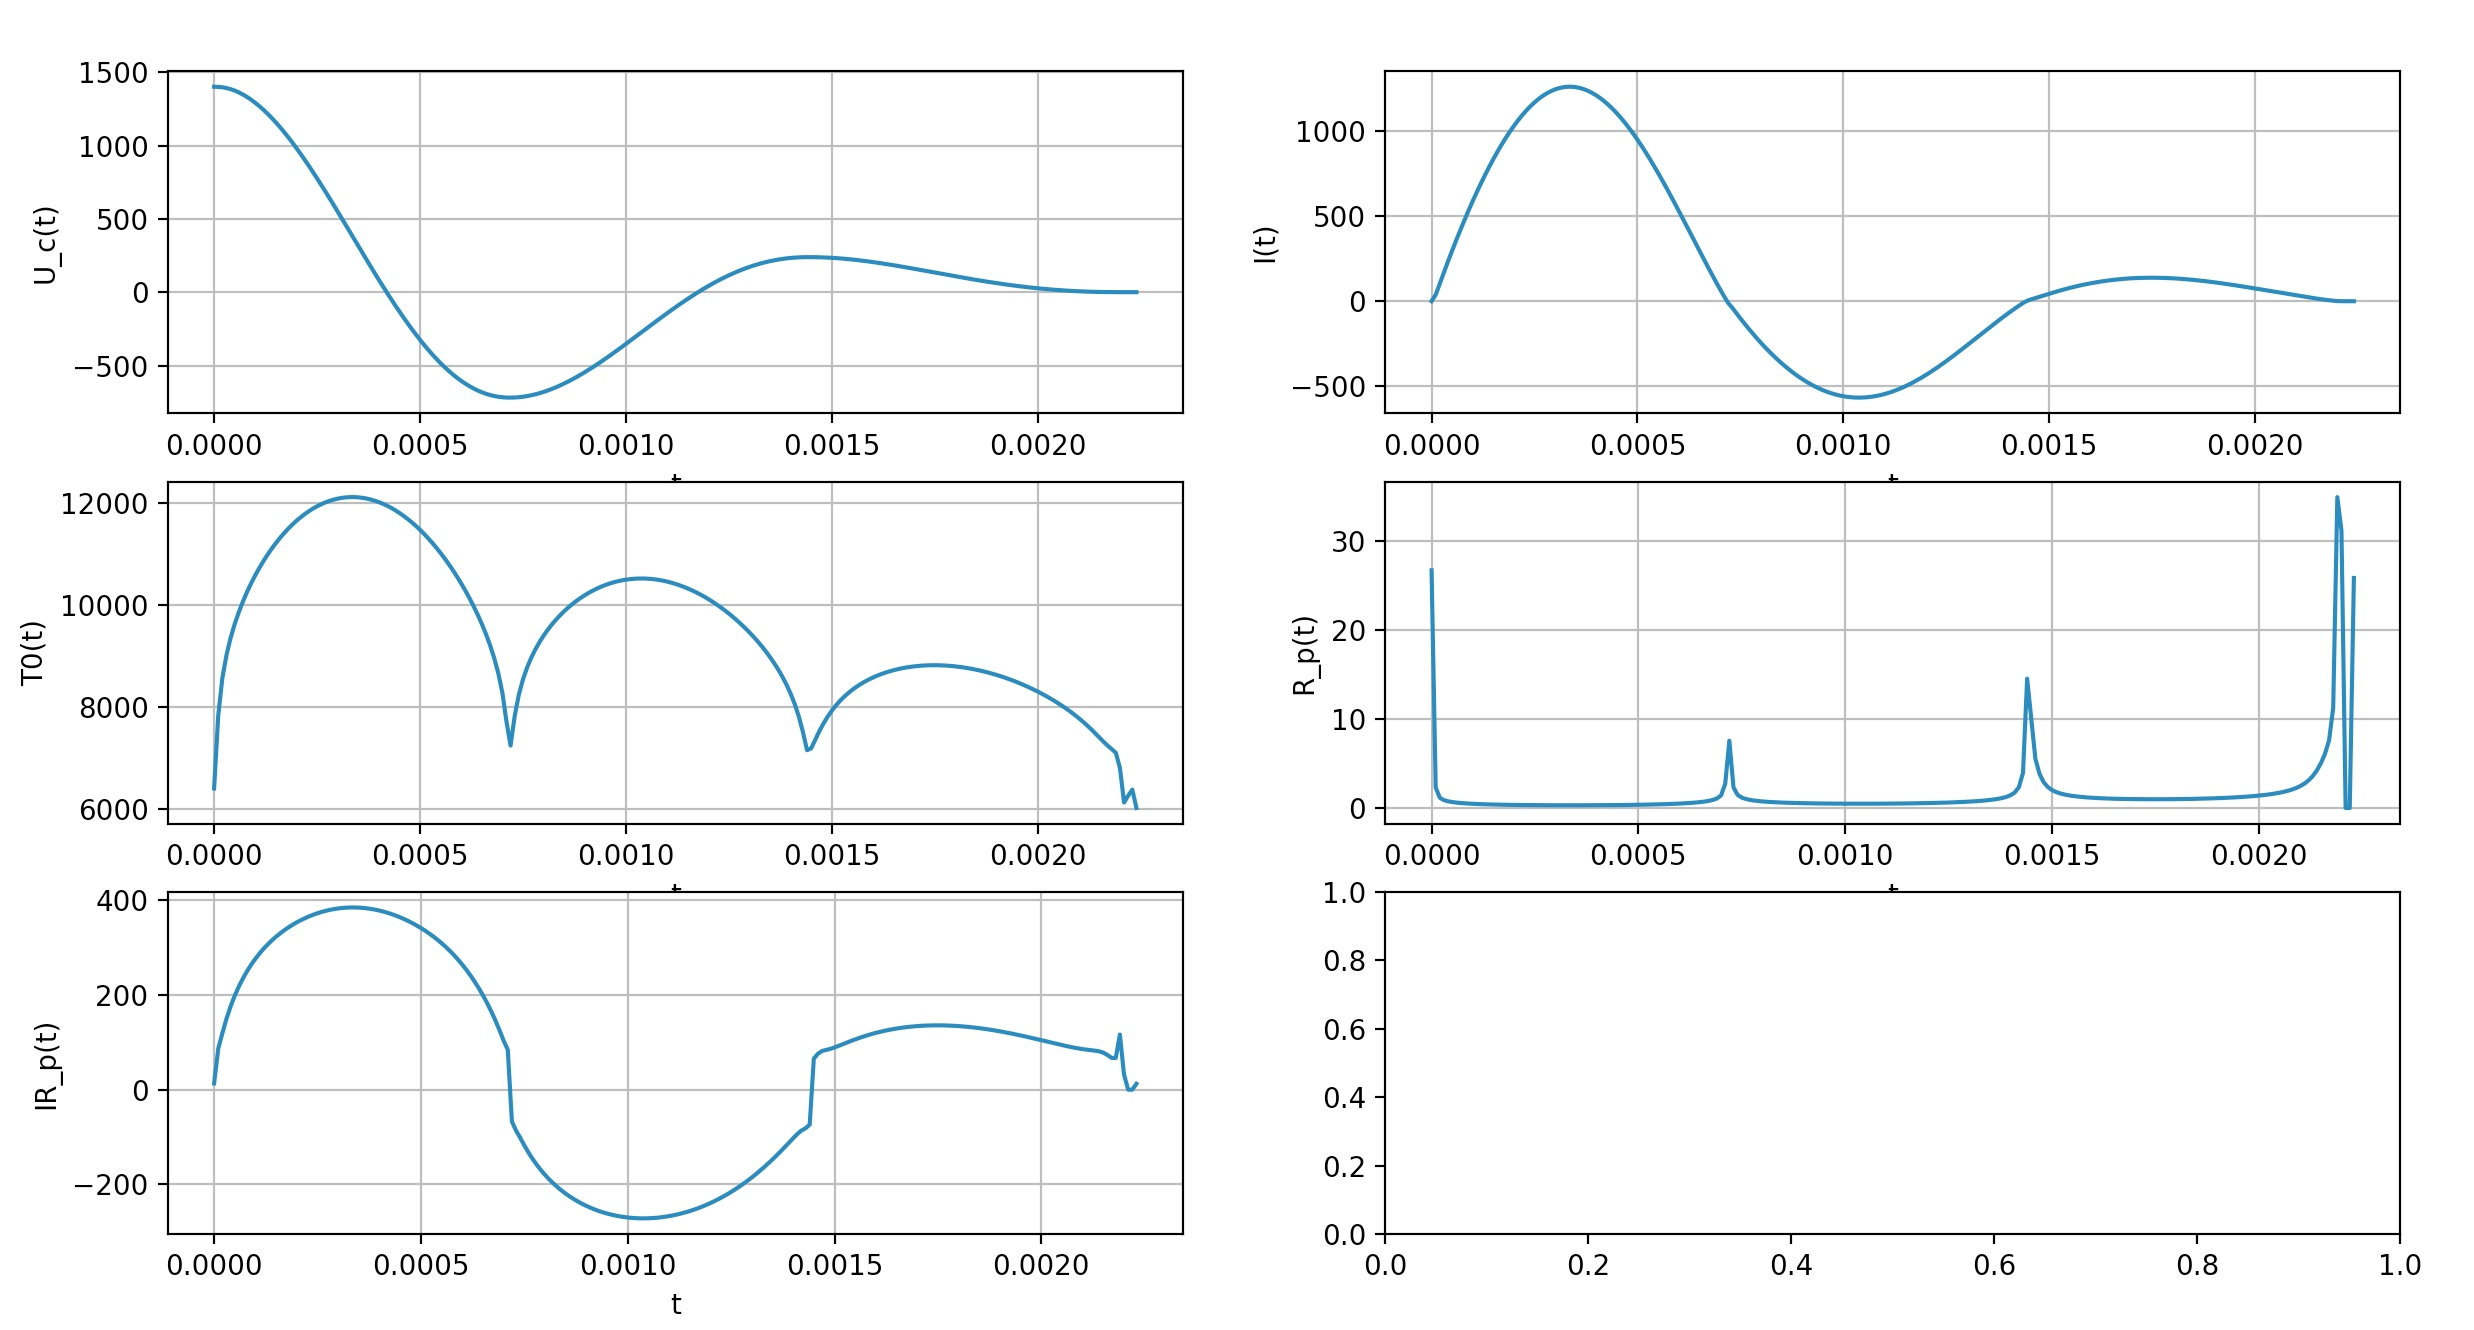
\includegraphics[scale = 0.2]{0.jpg}}
		\label{700}
	\end{center}
\end{figure}


\section{Листинг кода}

\begin{lstlisting}[label=lst1,caption=Реализация метода Рунге-Кутта 4-ого порядка точности]
from interpolation import *

from math import *


def calc_temperature(t0, t_w, m, z):
	return t0 + (t_w - t0) * (z ** m)



def calc_integral_func(z, sigma_from_temperature, t_w, t0, m):
	return z * calculate_value(sigma_from_temperature, calc_temperature(t0, t_w, m, z))



def calc_integral_by_trap_method(sigma_from_temperature, t_w, t0, m):
	n, b, a = 1000, 1, 0
	h = (b - a) / n
	
	result = calc_integral_func(b, sigma_from_temperature, t_w, t0, m)
	
	a += h
	while (a < b):
		result += 2 * calc_integral_func(a, sigma_from_temperature, t_w, t0, m)
		a += h
	
	return result * h




def calc_r_p(l_e, r, sigma_from_temperature, t_w, t0, m):
	result = l_e / (2 * pi * r * r)
	result /= calc_integral_by_trap_method(sigma_from_temperature, t_w, t0, m)
	return result



def calc_f(i, u_c, r_k, l_k, r_p):
	return (u_c - (r_k + r_p) * i) / l_k
	#return u_c / l_k


def calc_phi(c_k, i):
	return -i / c_k

def calc_k_q_values(h_t, i, u_c, r_k, l_k, c_k, r_p):
	k, q = [], []
	k1 = h_t * calc_f(i, u_c, r_k, l_k, r_p)
	q1 = h_t * calc_phi(c_k, i)
	
	k2 = h_t * calc_f(i + k1 / 2, u_c + q1 / 2, r_k, l_k, r_p)
	q2 = h_t * calc_phi(c_k, i + k1 / 2)
	
	k3 = h_t * calc_f(i + k2 / 2, u_c + q2 / 2, r_k, l_k, r_p)
	q3 = h_t * calc_phi(c_k, i + k2 / 2)
	
	k4 = h_t * calc_f(i + k3, u_c + q3, r_k, l_k, r_p)
	q4 = h_t * calc_phi(c_k, i + k3)
	
	k.append(k1)
	k.append(k2)
	k.append(k3)
	k.append(k4)
	
	q.append(q1)
	q.append(q2)
	q.append(q3)
	q.append(q4)
	
	return k, q


def runge_kutta_part(k, y_n):
	return y_n + (k[0] + 2 * k[1] + 2 * k[2] + k[3]) / 6


def calc_runge_kutta_fourth(k, q, i, u_c):
	return runge_kutta_part(k, i), runge_kutta_part(q, u_c)


def calc_values(d):
	result = []
	u_c = d.get("U_c")
	i = d.get("I")
	time = d.get("Time")
	l_e = d.get("L_e")
	r = d.get("R")
	t_w = d.get("T_w")
	r_k = d.get("R_k")
	l_k = d.get("L_k")
	c_k = d.get("C_k")
	
	
	t0_from_i = interp(d.get("I_T_0_m"), 0, 1)
	m_from_i = interp(d.get("I_T_0_m"), 0, 2)
	
	
	sigma_from_temperature = interp(d.get("T_sigma"), 0, 1)
	
	t0 = calculate_value(t0_from_i, log2(i))
	m = calculate_value(m_from_i, log2(i))
	
	r_p = calc_r_p(l_e, r, sigma_from_temperature, t_w, t0, m)
	
	
	result.append([u_c, i, t0, r_p, time[0]])
	
	
	for j in range(len(time) - 1):
		h_t = (time[j + 1] - time[j])
	
		k, q = calc_k_q_values(h_t, i, u_c, r_k, l_k, c_k, r_p)
		
		i, u_c = calc_runge_kutta_fourth(k, q, i, u_c)
		
		
		t0 = calculate_value(t0_from_i, log2(fabs(i)))
		m = calculate_value(m_from_i, log2(fabs(i)))
		r_p = calc_r_p(l_e, r, sigma_from_temperature, t_w, t0, m)
		
		result.append([u_c, i, t0, r_p, time[j + 1]])
	
	return result
\end{lstlisting}



\end{document}